\part{Sockets and Wireshark}
\section{Write a client program / script to send your username to each of tese servers and print the response received}
\begin{normalsize}
For each of the servers, a seperate script was used, albeit largely the same process. These scripts are referred to as TCP.py and UDP.py
\end{normalsize}

\definecolor{mygreen}{rgb}{0,0.6,0}

\lstinputlisting[style=python]{TCP.py}
\newpage
\lstinputlisting[style=python]{UDP.py}
\begin{normalsize}
The text returned by each server is included below.
\end{normalsize}
\begin{lstlisting}[breaklines, frame=single, title=TCP, numbers=left]
RESTART: C\Users:Elliot\Google Drive\Uni\Coursework\Distributed Systems and Networks\Python\TCP.py
Starting up socket on port 5002.
Response: Hello ep1e16, the date is 01/11/17 your code: qnpn
\end{lstlisting}
\begin{lstlisting}[breaklines, frame=single, title=UDP, numbers=left]
RESTART: C\Users:Elliot\Google Drive\Uni\Coursework\Distributed Systems and Networks\Python\UDP.py
Starting up socket on port 5005.
Response : Hello ep1e16, the date is 01/11/17
\end{lstlisting}
\section{Use a suitable capture filter in Wireshark to capture an interaction with the server.}
\begin{normalsize}
Below is a screenshot of said interaction. The interaction captures the client-server handshake (SYN, SYN-ACK, ACK), then the client pushing data to the server, the servers acknowledgement, then the closing of the socket by the server (PSH, ACK, FIN). The client acknowledges that the socket is closed, and the program ends. Included below is a screenshot of the wireshark capture, as well as the complete log of the capture. The capture filter used was:
\end{normalsize}
\begin{center}
\begin{tabular}{c}
\begin{lstlisting}
tcp port == 5002
\end{lstlisting}
\end{tabular}
\end{center}
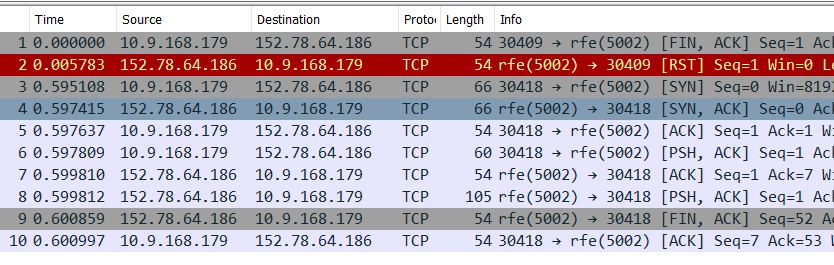
\includegraphics[scale=0.9]{wireshark_capture}

\section{What do you notice about the two interactions? How many packets are involved?}
\begin{normalsize}
In the complete transaction (ignoring the FIN,ACK and RST signals from the previous transfer), there are 8 packets involved. Three for the handshake (SYN, SYNACK, ACK), then two for the initial username transfer (PSH, ACK and ACK). The server then returns its response with PSH,ACK, followed by a FIN ACK packet. The client acknowledges this, and the connection ends. Note that the response transfer uses only three packets to return the string, and pass the FIN flag, with a combined acknowledgement from the client for both packets. 
\end{normalsize}

\lstinputlisting[style=python]{output.txt}



